\documentclass[a4paper,11pt]{article}

\usepackage{amsmath}
\usepackage{amssymb}
%\usepackage{amsthm}
\usepackage{graphicx}
\usepackage{epstopdf}
\epstopdfsetup{update}
%\usepackage{caption}
%\usepackage{subcaption}

\newcommand{\ba}{\begin{array}}
\newcommand{\ea}{\end{array}}

\newcommand{\bea}{\begin{eqnarray}}
\newcommand{\eea}{\end{eqnarray}}

\newcommand{\bc}{\begin{center}}
\newcommand{\ec}{\end{center}}

\newcommand{\ds}{\displaystyle}

\newcommand{\bt}{\begin{tabular}}
\newcommand{\et}{\end{tabular}}

\newcommand{\bi}{\begin{itemize}}
\newcommand{\ei}{\end{itemize}}

\newcommand{\bd}{\begin{description}}
\newcommand{\ed}{\end{description}}

\newcommand{\bp}{\begin{pmatrix}}
\newcommand{\ep}{\end{pmatrix}}

\newcommand{\pd}{\partial}
\newcommand{\sech}{\mbox{sech}}

\newcommand{\cf}{{\it cf.}~}

\newcommand{\ltwo}{L_{2}(\mathbb{R}^{2})}
\newcommand{\smooth}{C^{\infty}_{0}(\mathbb{R}^{2})}

\newcommand{\br}{{\bf r}}
\newcommand{\bk}{{\bf k}}
\newcommand{\bv}{{\bf v}}

\newcommand{\gnorm}[1]{\left|\left| #1\right|\right|}
\newcommand{\ipro}[2]{\left<#1,#2 \right>}

\author{Christopher W. Curtis \\
Ricardo Carretero\\
Matteo Polimeno}
\date{}
\title{Characterizing Coherent Structures in Bose-Einstein Condensates through Dynamic-Mode Decomposition}
\begin{document}
\maketitle
\section*{Introduction}
With the recent experimental observation of turbulent cascades in a Bose-Einstein Condensate (BEC) \cite{navon}, it is important to continue to better understand and characterize in as quantitative a means as possible the complex dynamics associated with turbulence in dispersive, nonlinear-wave systems.  While small-amplitude states whose statistics remain nearly Gaussian permit a relatively complete analytic characterization of turbulent cascades, embodied in the weak-wave turbulence (WWT) theory initiated in \cite{zakharov} and collected in \cite{nazarenko}, as noted in \cite{newell,cai}, the assumptions which one makes to derive results in WWT necessarily must generically break down over long-enough timescales.  

This breakdown is best characterized by the formation of long-wavelength, larger-amplitude coherent structures (CSs).  In classic, one-dimensional systems, characterizing such structures in terms of solitons is relatively straightforward; see \cite{cai}.  However, in two-dimensions, and for systems like the defocusing nonlinear Schr\"{o}dinger equation (NLSE), describing coherent structures in quantitative terms is far more challenging.  In the context of BECs, a variety of heuristic metrics to characterize CSs appeared in \cite{nazarenko2}.  In the broader context of WWT, along with classic approaches built around studying qualitative features in Fourier transforms, methods based on tracking spikes in Gaussian curvature of the solution have appeared in \cite{mordant}.  

However, as noted in \cite{nazarenko2}, CSs are difficult to visulalize in terms of physically measurable variables in BECs.  This is due in part to the role that vortices play in BECs, whereby the formation of CSs corresponds to the elimination of vortices.  This in some sense removes the most readily identifiable features of the flow, making characterization of the transition away from the WWT state difficult.  In this paper, instead, we study the use of Dynamic-Mode Decompositions (DMDs), \cite{schmid,williams,kutz}, which is a modal decomposition generated by discrete snap-shots of the temporal evolution of the BEC.  The advantage of DMDs is in their great flexibility due to their essentially being a model-free means of analyzing flows.  

As we show, by selecting the most temporally dominant modes from the DMD, we are readily able to characterize coherent states that otherwise remain undetectable in the BEC flow.  

\section*{Modelling and Weak-Wave Turbulence}

In non-dimensional coordinates (see the Appendix for details on the non-dimensionalization), we model the BEC through the use of a stochastically forced Gross--Pitaevskii (GP), or NLS, equation 
\[
i\psi_{t} = -\Delta \psi +  \left| \psi\right|^{2}\psi + \gamma_{f}({\bf x},t) - i(\nu_{h}\Delta^{2n}+\nu_{l}\tilde{\Delta}^{-2n})\psi, ~ \psi({\bf x},0)=0.
\]
Note, we always remain in the defocusing, or `dark', case.  We solve this equation with periodic boundary conditions, where the common period $2L \gg 1$ so that we have the equivalent Fourier representation of $\psi$,
\[
\psi({\bf x},t) = \sum_{{\bf k}_{mn}} a({\bf k}_{mn},t) e^{\pi i {\bf k}_{mn}\cdot {\bf x}/L}.
\]

The forcing $\gamma_{f}$ is chosen so as to be a spectrally-band limited function 
\[
\gamma_{f}({\bf x},t) = \gamma_{0}e^{2\pi i\varphi(t)}\sum_{k_{l}\leq |{\bf k}_{mn}| \leq k_{h}} e^{\pi i {\bf k}_{mn}\cdot {\bf x}/L}, ~ {\bf k}_{mn} = (m,n), 
\]
and the phase $\varphi(t)$ is such that $\varphi(t)  \sim U(0,1)$ where $U(0,1)$ denotes random variables uniformly distributed between $0$ and $1$.  Thus, our forcing is characterized by an injection range of wavenumbers via the choices of $k_{l}$ and $k_{h}$.  We likewise see that the forcing is unbiased in any particular spatial direction, so that by starting with zero-initial conditions, we see that the solution $\psi({\bf x},t)$ will largely mimick the forcing until it has reached a large enough amplitude that nonlinearity, through four-wave mixing, is able to transfer energy across Fourier modes.  This is ultimately balanced against the strength of the hyperviscosity characterized by the magnitude of $\nu_{h}$ and the hypoviscosity characterized by the magnitude of $\nu_{l}$.  

We note that the question of what a `large' domain is is somewhat ambiguous in this problem due to the forcing.  Traditionally when modelling a BEC, a length scale is set via the `healing-length' \cite{pethick}, which ultimately determines the width of vortices in the GPE.  However, to do this one must have a fixed particle number $N= \int \left|\psi\right|^{2}d{\bf x}$, but due to the forcing we necessarily have that 
\begin{align*}
\frac{1}{2}\frac{dN}{dt} = &  \mbox{Im}\left\{\int \gamma_{f}({\bf x},t) \psi^{\ast} d{\bf x} \right\}\\
& - \int \psi^{\ast}\left(\nu_{h}\Delta^{2n}+\nu_{l}\tilde{\Delta}^{-2n}\right)\psi d{\bf x}
\end{align*}
so that the particle number, and thus length scale, can change with time.  Ultimately though, a quasi-equilibrium is achieved through the balance of injection due to the forcing $\gamma_{f}$ and the particle removal/energy dissipation due to the hyper/hypoviscosity.  

By forcing the system starting from a zero-amplitude state, we hope to ultimately generate a weak-wave turbulence (WWT) state.  This is characterized as a nontrivial energy flux in wavenumber.  The associated isotropic energy density $E_{d}(k,t)$ is given by 
\[
E_{d}(k,t) = 2\pi k\omega(k)n(k,t), 
\]
where $\omega(k)$ is the dispersion relationship of the GPE, and $n(k)$ is given by 
\[
n(k,t) = \left< \left|a(\bk_{nm},t)\right|^{2}\right>, ~ \left|\bk_{nm}\right| = k.
\]
The brackets denote averaging, which in our case, assuming ergodicity, will correspond to temporally averaging the power spectra of the solution of the GPE.  

Associated with the energy density is an affiliated energy flux $\epsilon$ so that 
\[
\pd_{t} E_{d} + \pd_{k}\epsilon \sim 0.
\]
It is one of the major achievements in the WWT theory that one can derive Boltzman like kinetic equations describing the evolution of $n(k,t)$ \cite{nazarenko}.  Thus, if we characterize the WWT state as one at which the energy density is in quasi-equilibrium so that $\pd_{t}E_{d}\sim 0$, which therefore implies that $\pd_{t}n(k,t)\sim 0$, we can then distinguish equilibrium profiles of $n(k,t)$ by whether $\epsilon \sim 0$ or $\epsilon \sim c$, where c is some constant.  The zero case corresponds to no energy flux, thereby describing a thermodynamically steady state associated with the equipartion of energy.  It is the non-zero energy flux states which distinguish WWT states, and those that we are most interested in studying.  

\section*{Dynamic-Mode Decomposition}
We briefly review the details of the DMD for completeness and to better explain later results.  In DMD, we assume that any time series of a dynamical quantity of interest, denoted by $\left\{\phi_{n}\right\}_{n=1}^{\infty}$, where $\phi_{n}\in \mathbb{R}^{M}$, can be described through a linear process mediated via an operator, say $A$ so that 
\[
\phi_{n+1} = A \phi_{n}.  
\] 
We treat $A$ as essentially unknowable in any direct sense, but by using the affiliated matrices $V_{1}^{N}$, where
\[
V^{N}_{1} = \left\{\phi_{1} \cdots \phi_{N} \right\}
\]
and $V_{2}^{N} = AV_{1}^{N}$, and using a Singular Value Decomposition (SVD) on $V_{1}^{N}$ so that $V_{1}^{N} = U\Sigma W^{\dagger}$, we see that 
\[
U^{\dagger}AU = \tilde{S}, ~ \tilde{S} = U^{\dagger}V_{2}^{N}W\Sigma^{-1}.
\]
Thus by computing the associated eigenvalues and eigenvectors of $\tilde{S}$, say $\mu_{j}$ and $\tilde{\phi}_{j}$ respectively, then for $N$ large enough with sufficiently controlled spacing in the time-series, these eigenvalues and eigenvectors will approximate those of $A$.  Likewise, this allows us to write each vector in our time-series as 
\[
\phi_{n} = \sum_{j=1}^{N} b_{j}\mu_{j}^{n} U\tilde{\phi}_{j} + {\bf r}_{n},
\]
where ${\bf r}_{n}$ denotes the residual at the $n^{th}$ sampling time. 
\section*{Characterizing Coherent States}

\subsection*{Methodology for Implementing the DMD}

In order to realize WWT regimes of the NLS equation, following \cite{nazarenko2}, we run each simulation over a domain of size $L=128$ with a total of $K_{T}=256$ modes in each spatial direction.  Using a two stage Runge-Kutta scheme with a time step of $\delta t=.1$, by simulating up to $t_{f}=1.5\times 10^{4}$, we are able to see the necessary turbulent or mixed dynamics that we are interested in.  

With regards to the DMD, we take as the ``observable" quantity the magnitude $|\psi(x,y,t)|$, which we sample every five numerical timesteps, so that the sampling rate $\delta t_{s}=.5$.  We begin sampling at $t_{f}=1.485\times10^{4}$, so that we sample the last $150$ units of time, thereby ensuring we are in fact performing DMD on a fully turbulent or mixed flow.  Thus, if we sample over the entire physical domain, this corresponds then to case where the dimensionality of the DMD vectors $M = 256^2 \gg 150/.5 = 300$, so that $M$ is far larger than the number of time samples taken. 

 Given the numerical limitations of looking at higher resolution sampling rates, we approach analyzing the results of the DMD method from two perspectives.  Letting $\lambda_{j} = \log \mu_{j}/\delta t_{s}$, and scaling the modes $\tilde{\phi}_{j}$ so they have vector-2 norm equal to one, we use the magnitudes of the real parts of $\lambda_{j}$ and the magnitude of the coefficients $b_{j}$ to guide the selection of the most `dominant' modes.  By comparing across these two sets of information, we can make informed, quantitatively supported decisions about what represents a more or less significant mode.  

\subsection*{Down-Scale Weak Turbulence Cascades}
In this case, we take $k_{l}=4$, $k_{h}=6$, and $\gamma_{0}=2.1\times 10^{-3}$.  To recreate the WWT results of \cite{nazarenko2}, we keep both hypo and hyperviscosity in place.  The results of this are seen in Figures \ref{fig:ampcompwwt} and \ref{fig:oscwwt}.  In particular, we see the fully evolved amplitude of the NLS equation at $t_{f}$, i.e. $|\psi(x,y,t_{f})|$, in Figure \ref{fig:ampcompwwt} (a) compared against the weighted mean of the flow computed via the DMD shown in  Figures \ref{fig:ampcompwwt} (b).  As seen, we can characterize the WWT regime in part by noting the lack of clear structure in the mean mode.  The finer details seen in Figure \ref{fig:ampcompwwt} (a) can in part be recovered by looking beyond the mean mode to higher oscillatory/weakly-transitory modes, seen in Figure \ref{fig:oscwwt}.  Note, by a plot of a weighted DMD mode, we mean that we plot $\left|b_{j}U\tilde{\phi}_{j}\right|$, thereby allowing us to visualize the spatial structure associated with the mode as well as its relative contribution controlled by the magnitude of $b_{j}$ since each mode $U\tilde{\phi}_{j}$ is scaled to have unit vector norm.  
\begin{figure}[!ht]
\centering
\begin{tabular}{cc}
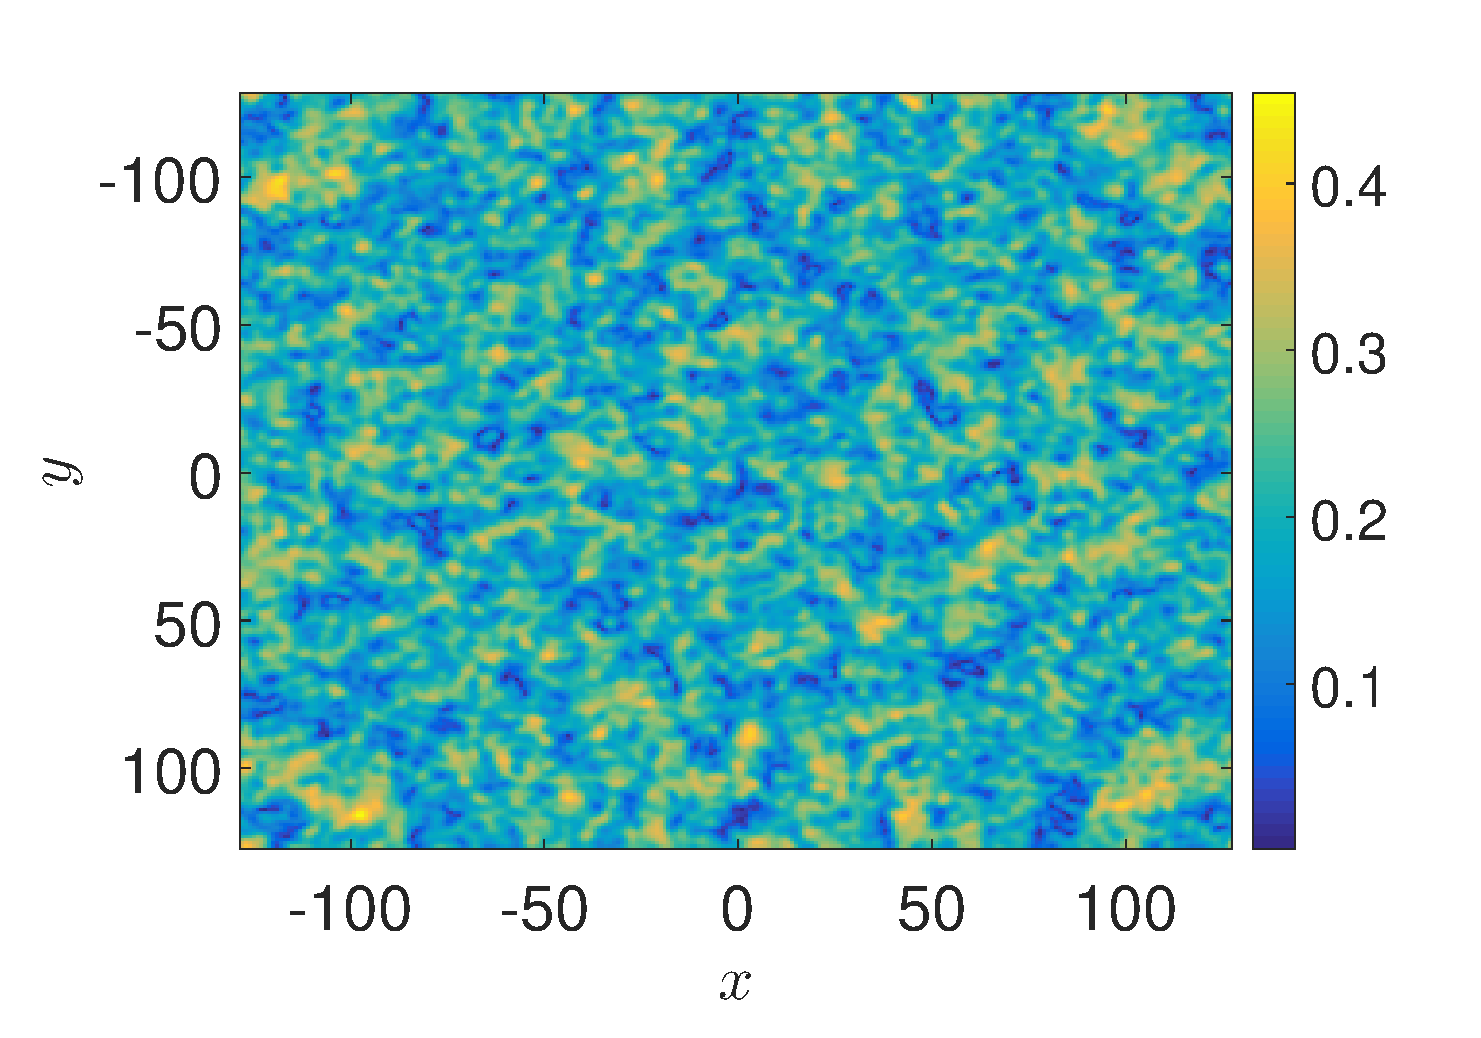
\includegraphics[width=.525\textwidth]{amplitude_wwt_K_128_Lx_128_tf_1pt5e4} &\hspace{-25pt} \includegraphics[width=.525\textwidth]{mean_wwtforce_K_128_Lx_128_tf_1_pt5e4} \\
(a) & (b)\\
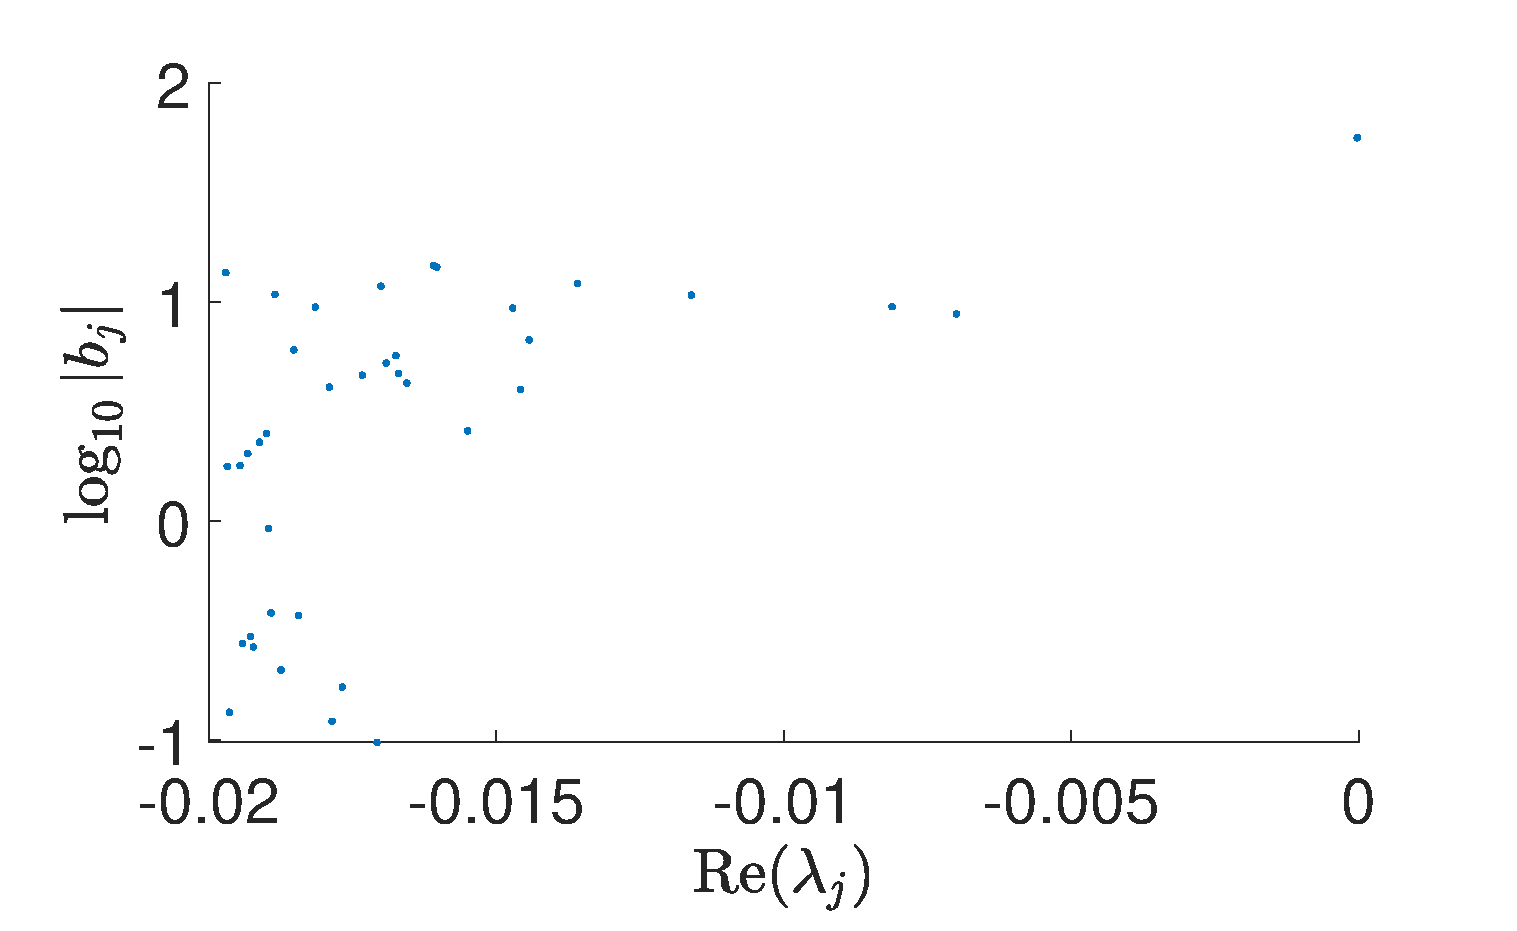
\includegraphics[width=.525\textwidth]{bvals_vs_real_lam_wwtforce_K_128_Lx_128_tf_1_pt5e4} &\hspace{-25pt} 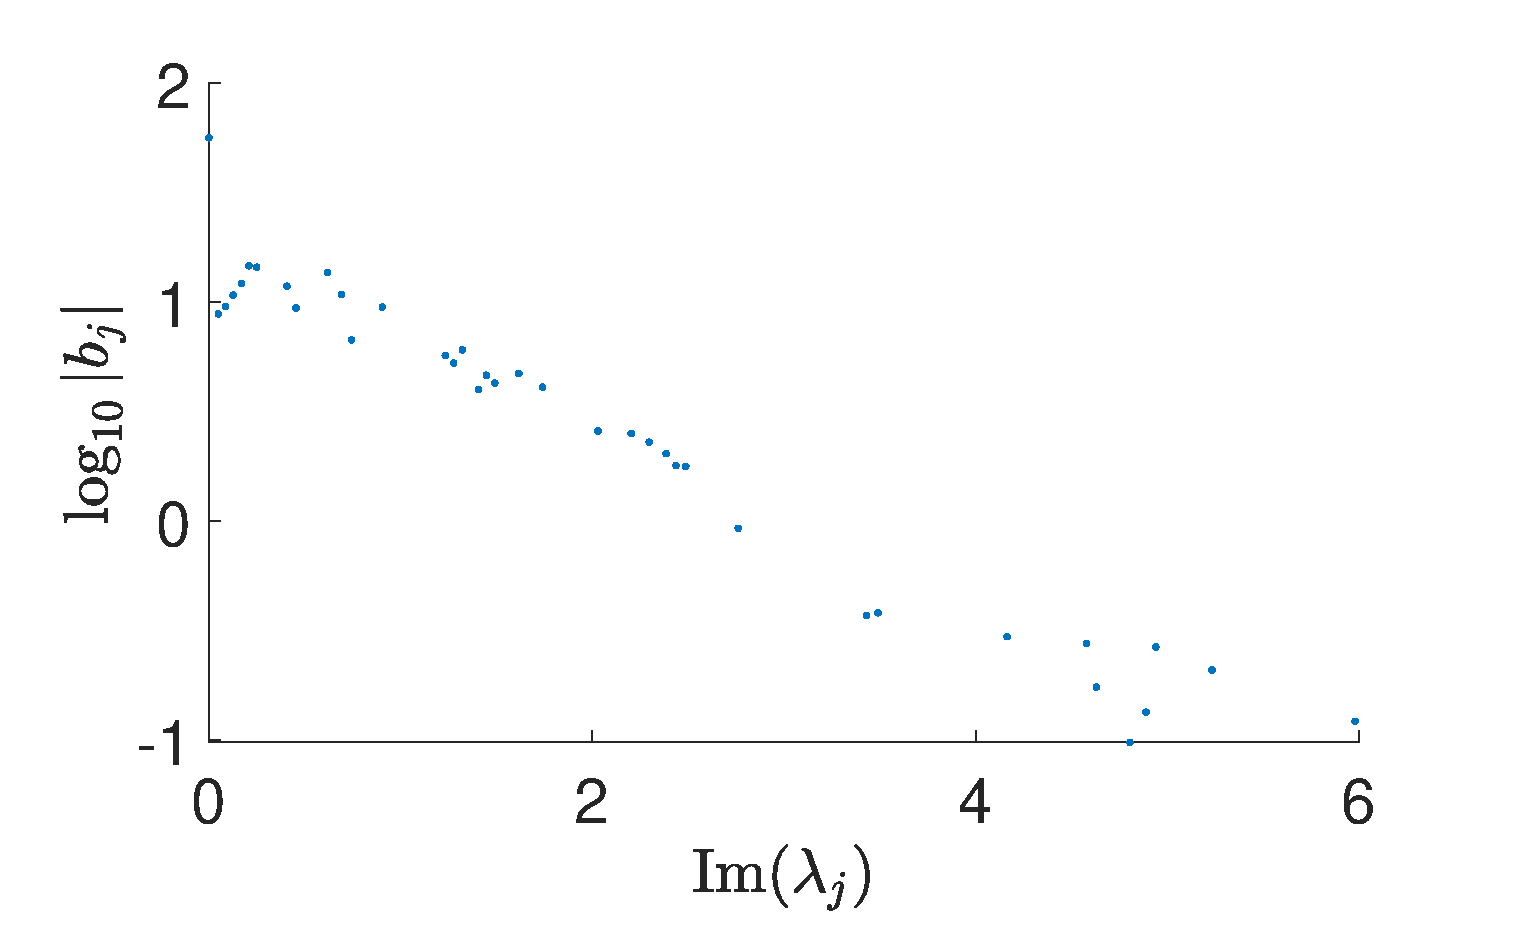
\includegraphics[width=.525\textwidth]{bvals_vs_imag_lam_wwtforce_K_128_Lx_128_tf_1_pt5e4}\\
(c) & (d)
\end{tabular}
\caption{The amplitude $\left|\psi(x,y,t_{f})\right|$ (a), weighted mean (b),  plot of $\log_{10}|b_{j}|$ against $\mbox{Re}(\lambda_{j})$ (c), and plot of $\log_{10}|b_{j}|$ against $\mbox{Im}(\lambda_{j})$ (d) for $k_{l}=4$, $k_{h}=6$, $\gamma_{0}=2.1\times 10^{-3}$. }
\label{fig:ampcompwwt}
\end{figure}
\begin{figure}[!ht]
\centering
\begin{tabular}{cc}
\includegraphics[width=.51\textwidth]{osc1_wwtforce_K_128_Lx_128_tf_1_pt5e4} &\hspace{-15pt} \includegraphics[width=.51\textwidth]{osc2_wwtforce_K_128_Lx_128_tf_1_pt5e4} \\
(a) & (b)\\
\includegraphics[width=.51\textwidth]{osc3_wwtforce_K_128_Lx_128_tf_1_pt5e4} &\hspace{-15pt} \includegraphics[width=.51\textwidth]{osc4_wwtforce_K_128_Lx_128_tf_1_pt5e4}\\
(c) & (d)
\end{tabular}
\caption{The first four, by magnitude in $|b_{j}|$, weighted oscillatory/weakly-transient modes for $k_{l}=4$, $k_{h}=6$, $\gamma_{0}=2.1\times 10^{-3}$. }
\label{fig:oscwwt}
\end{figure}

As seen in  Figure \ref{fig:ampcompwwt} (c), among those modes which are weakly-transitory, defined by focusing only on those DMD modes such that $\mbox{Re}(\lambda_{j})\geq-.02$, the mean is the dominant mode with respect to its magnitude of $|b_{j}|$.  We see a relatively uniform distribution of the magnitudes of $|b_{j}|$ against $\mbox{Im}(\lambda_{j})$, showing us a kind of temporal Fourier transform in which we see higher frequencies corresponding to smaller values of $|b_{j}|$.  Note the matrices involved in the DMD are all real in our case, and thus we only plot against those $\lambda_{j}$ with positive real part since we have symmetry across the real line.  

\subsection*{Long-Wavelength Saturation and Coherent States}
Through the remaining simulations, we remove the hypoviscosity, and let $\gamma_{0}=1.6\times 10^{-3}$, thereby allowing for saturation in longer-wavelengths to occur.  If we continue to look at the relatively low frequency forcing explored above, we expect to see long-wavelength coherent structures to form.  It is at this point that we can plainly see the advantage of using the DMD by comparing the fully evolved solution to the NLS equation in Figure \ref{fig:ampcomplf} (a) to the mean DMD mode in Figure \ref{fig:ampcomplf} (b).  We see in Figure \ref{fig:ampcomplf} (c) that this mode also has the largest associated value of $|b_{j}|$, so that, taking into account all other modes being oscillatory/weakly-transitory, the condensed state seen in the mean represents a kind of temporal limit of the dynamics.  The mean mode clearly identifies a finite number of vortices interacting through a finite amplitude background.  
\begin{figure}[!ht]
\centering
\begin{tabular}{cc}
\includegraphics[width=.525\textwidth]{amplitude_lfforce_K_128_Lx_128_tf_1pt5e4} &\hspace{-25pt} \includegraphics[width=.525\textwidth]{mean_lfforce_K_128_Lx_128_tf_1_pt5e4} \\
(a) & (b)\\
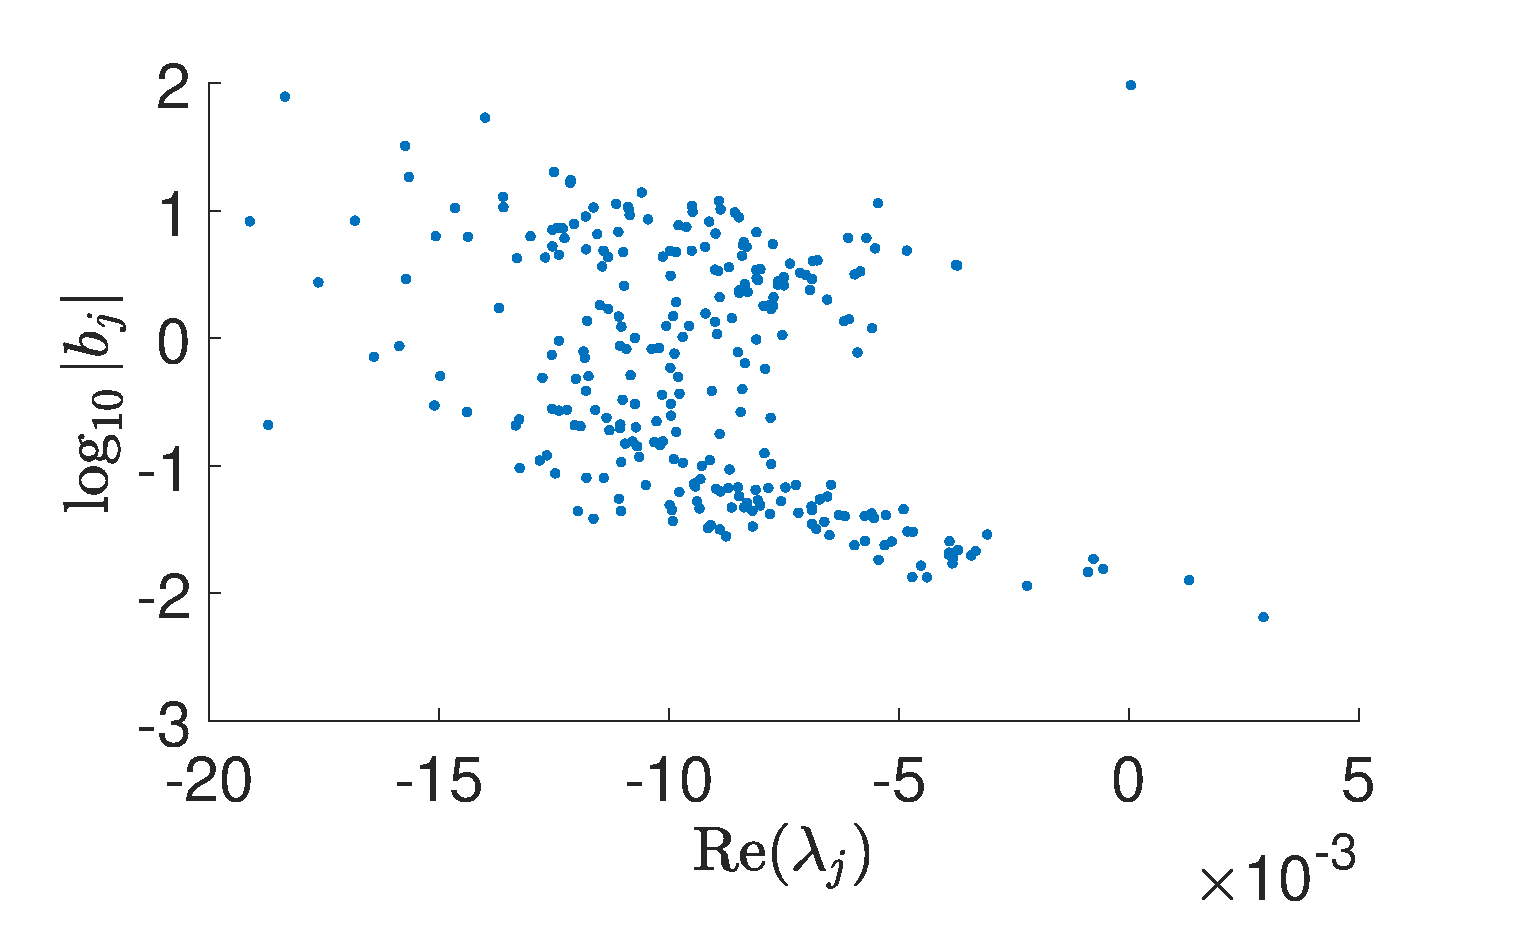
\includegraphics[width=.525\textwidth]{bvals_vs_real_lam_lfforce_K_128_Lx_128_tf_1_pt5e4} &\hspace{-25pt} 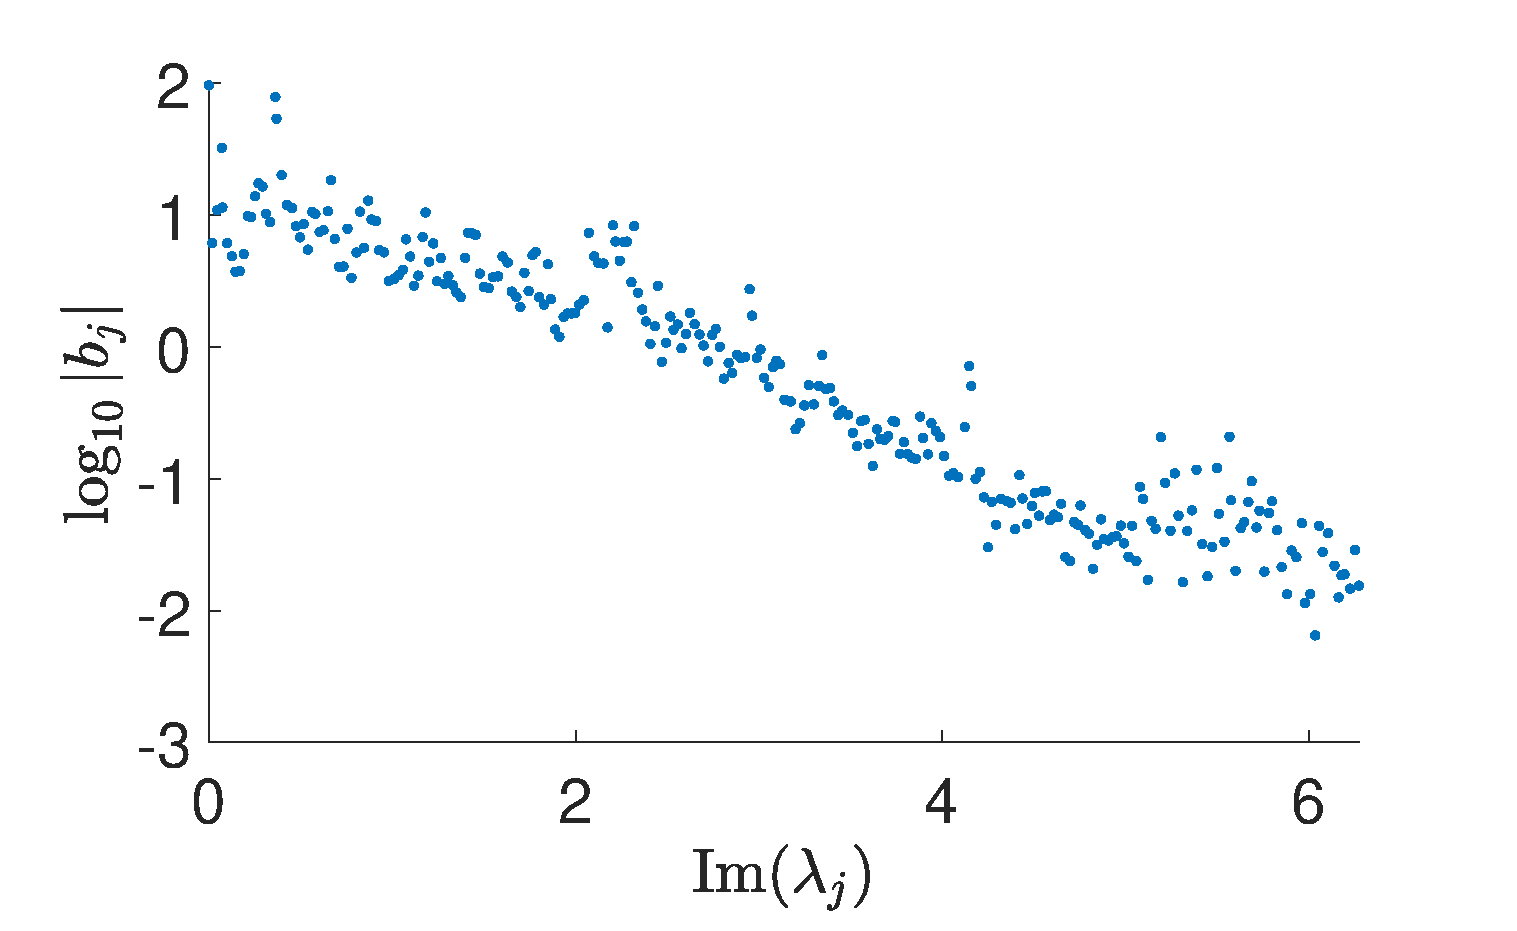
\includegraphics[width=.525\textwidth]{bvals_vs_imag_lam_lfforce_K_128_Lx_128_tf_1_pt5e4}\\
(c) & (d)
\end{tabular}
\caption{The amplitude $\left|\psi(x,y,t_{f})\right|$ (a), weighted mean (b),  plot of $\log_{10}|b_{j}|$ against $\mbox{Re}(\lambda_{j})$ (c), and plot of $\log_{10}|b_{j}|$ against $\mbox{Im}(\lambda_{j})$ (d) for $k_{l}=4$, $k_{h}=6$, $\gamma_{0}=1.6\times 10^{-3}$. }
\label{fig:ampcomplf}
\end{figure}
\begin{figure}[!ht]
\centering
\begin{tabular}{cc}
\includegraphics[width=.51\textwidth]{osc1_lfforce_K_128_Lx_128_tf_1_pt5e4} &\hspace{-15pt} \includegraphics[width=.51\textwidth]{osc2_lfforce_K_128_Lx_128_tf_1_pt5e4} \\
(a) & (b)\\
\includegraphics[width=.51\textwidth]{osc3_lfforce_K_128_Lx_128_tf_1_pt5e4} &\hspace{-15pt} \includegraphics[width=.51\textwidth]{osc4_lfforce_K_128_Lx_128_tf_1_pt5e4}\\
(c) & (d)
\end{tabular}
\caption{The first four, by magnitude in $|b_{j}|$, weigthed oscillatory/weakly-transient modes for $k_{l}=4$, $k_{h}=6$, $\gamma_{0}=1.6\times 10^{-3}$. }
\label{fig:osclf}
\end{figure}

Moreover, we see from Figure \ref{fig:ampcomplf} (d) that the higher temporal frequencies of oscillation correspond to far smaller magnitudes of $|b_{j}|$ than in the WWT regime examined above, so that the dynamics is characterized by slower oscillating modes than in the WWT regime.  The finer spatial dynamics can be seen in part by examining the plots in Figure \ref{fig:osclf}.  

We now look at higher-frequency forcing where we let $k_{l}=60$ and $k_{h}=63$.  As in the low-frequency, long-wavelength saturated case above, we see that the mean DMD mode seen in Figure \ref{fig:ampcomphf} clearly isolates the condensed dynamics obscured through the higher-frequency spatial features in the solution to the NLS equation seen in Figure \ref{fig:ampcomphf} (a).  In contrast the low-frequency forcing case above though, we see in the oscillatory/weakly-transitory modes in Figure \ref{fig:oschf}, spatial dynamics with far sharper, or higher-frequency, spatial features, thus clearly reflecting the different forcing mechanism in play in this simulation.   
\begin{figure}[!ht]
\centering
\begin{tabular}{cc}
\includegraphics[width=.51\textwidth]{amplitude_hfforce_K_128_Lx_128_tf_1pt5e4} &\hspace{-15pt} 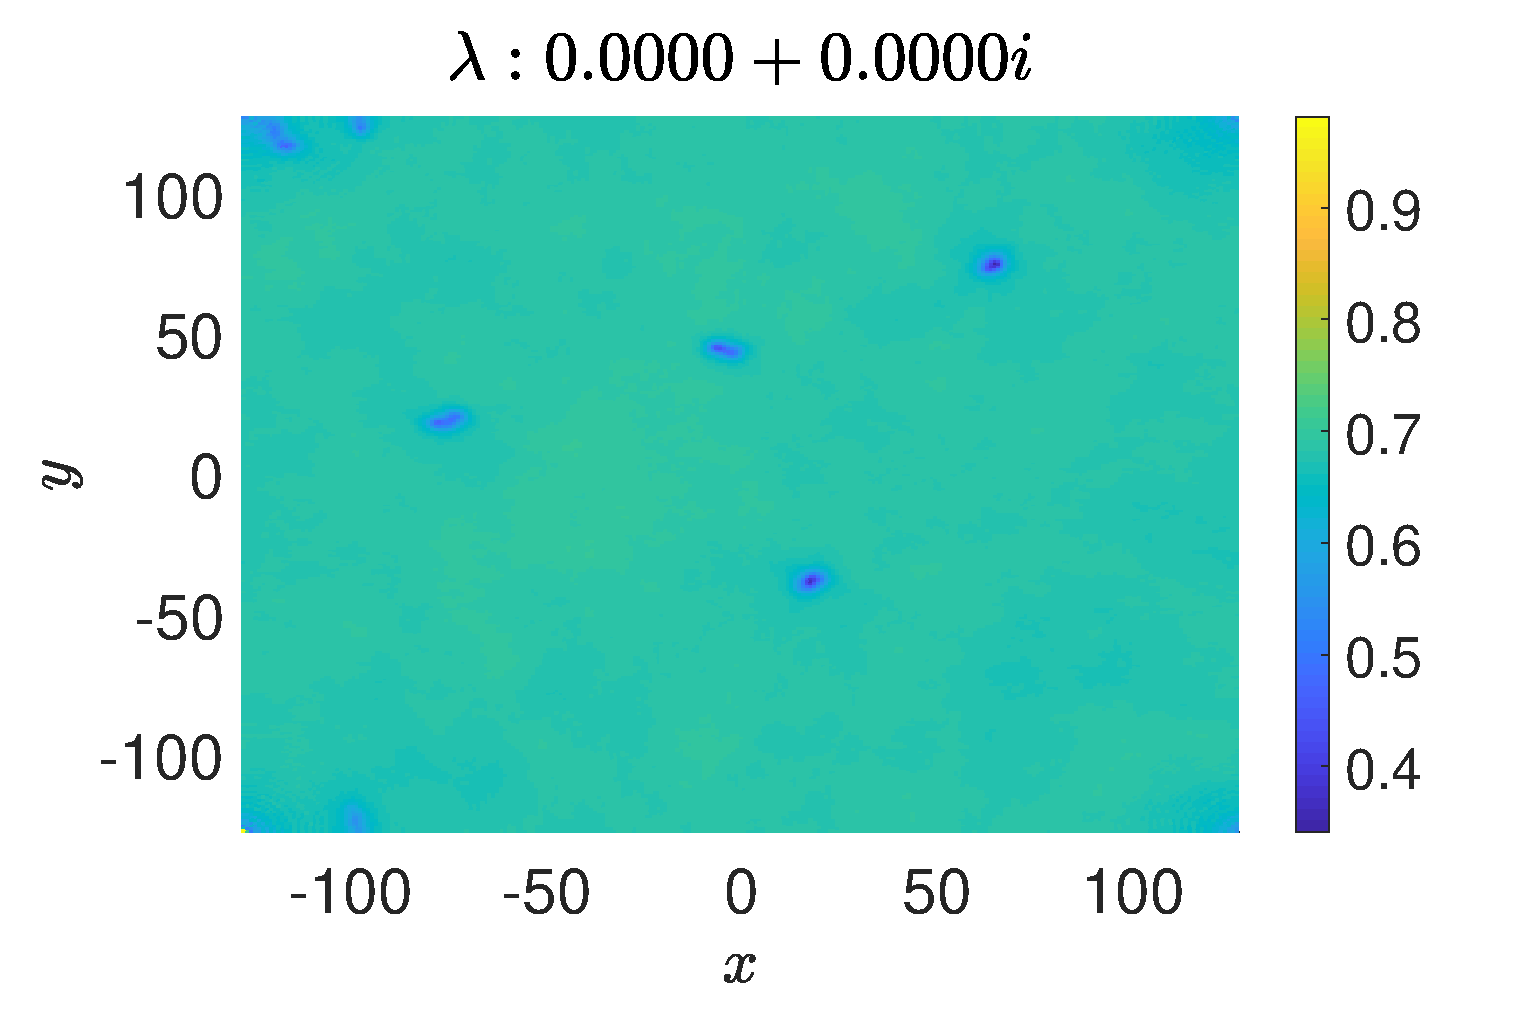
\includegraphics[width=.51\textwidth]{mean_hfforce_K_128_Lx_128_tf_1_pt5e4} \\
(a) & (b)\\
\includegraphics[width=.51\textwidth]{bvals_vs_real_lam_hfforce_K_128_Lx_128_tf_1_pt5e4} &\hspace{-15pt} 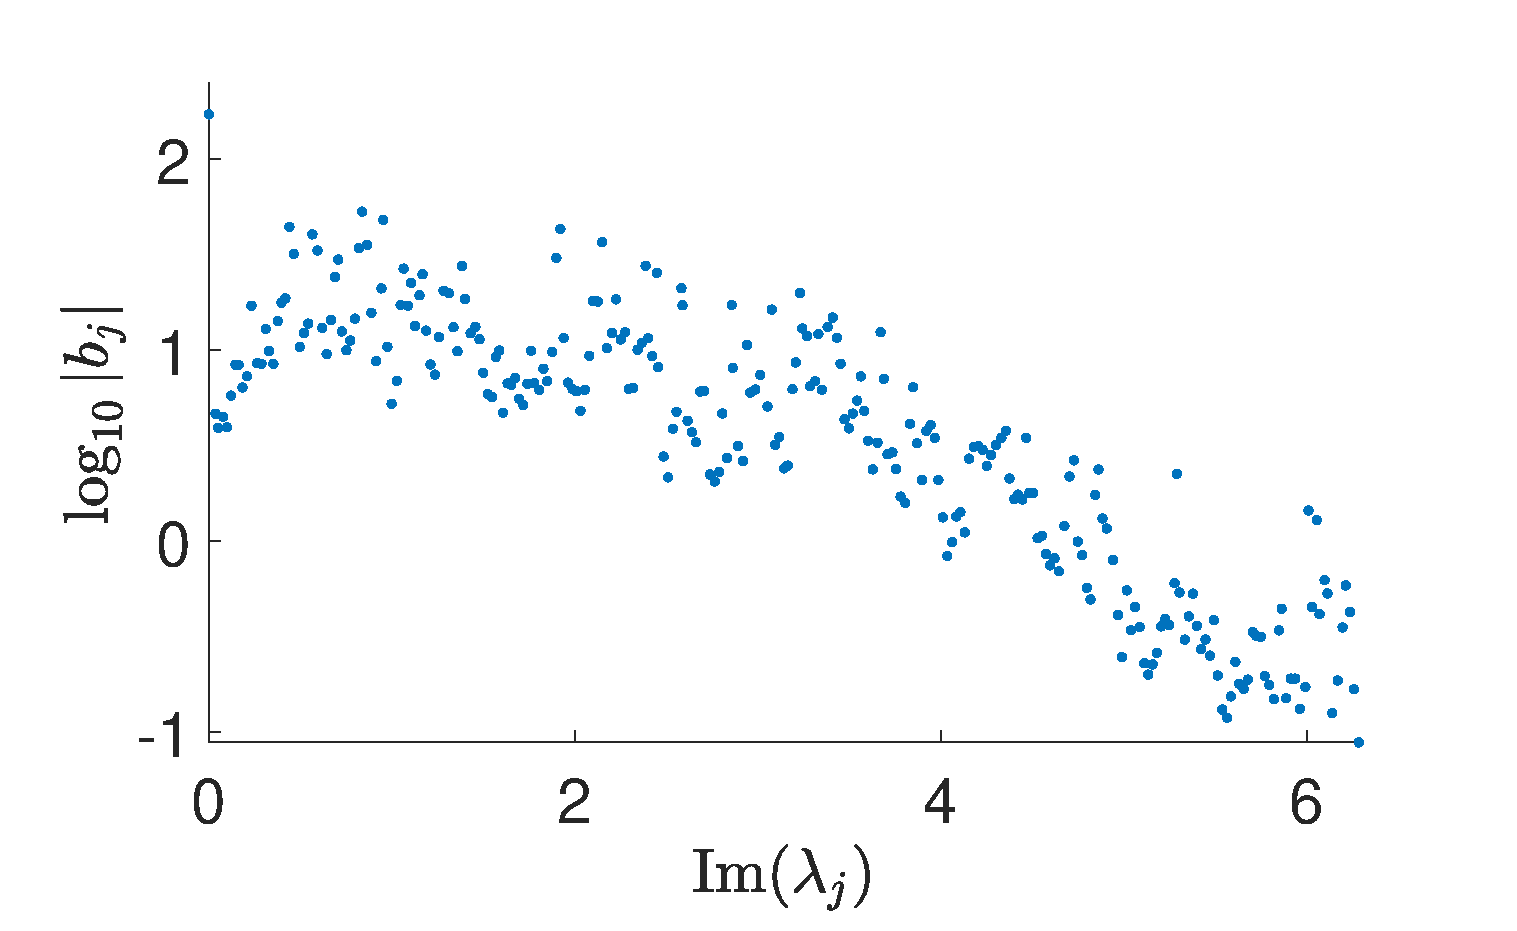
\includegraphics[width=.51\textwidth]{bvals_vs_imag_lam_hfforce_K_128_Lx_128_tf_1_pt5e4}\\
(c) & (d)
\end{tabular}
\caption{The amplitude $\left|\psi(x,y,t_{f})\right|$ (a), weighted mean (b),  plot of $\log_{10}|b_{j}|$ against $\mbox{Re}(\lambda_{j})$ (c), and plot of $\log_{10}|b_{j}|$ against $\mbox{Im}(\lambda_{j})$ (d) for $k_{l}=60$, $k_{h}=63$, $\gamma_{0}=1.6\times 10^{-3}$. }
\label{fig:ampcomphf}
\end{figure}
\begin{figure}[!ht]
\centering
\begin{tabular}{cc}
\includegraphics[width=.51\textwidth]{osc1_hfforce_K_128_Lx_128_tf_1_pt5e4} &\hspace{-15pt} \includegraphics[width=.51\textwidth]{osc2_hfforce_K_128_Lx_128_tf_1_pt5e4} \\
(a) & (b)\\
\includegraphics[width=.51\textwidth]{osc3_hfforce_K_128_Lx_128_tf_1_pt5e4} &\hspace{-15pt} \includegraphics[width=.51\textwidth]{osc4_hfforce_K_128_Lx_128_tf_1_pt5e4}\\
(c) & (d)
\end{tabular}
\caption{The first four, by magnitude in $|b_{j}|$, weighted oscillatory/weakly-transient modes $k_{l}=60$, $k_{h}=63$, $\gamma_{0}=1.6\times 10^{-3}$. }
\label{fig:oschf}
\end{figure}

\section*{Conclusion}

\section*{Appendix}
With units, our model of a BEC is given by the following Gross--Pitaevksii equation (GPE)
\[
i\hbar\psi_{t} = -\frac{\hbar^{2}}{2m}\Delta \psi + g\left| \psi\right|^{2}\psi, ~ g = \frac{4\pi \hbar^{2}a_{s}}{m}
\]
where $a_{s}$ is the `scattering length', and with the clear understanding that $\left|\psi\right|^{2}dxdy$ describes probabilities in the sense that 
\[
\int |\psi|^{2}dxdy = N,
\]
where we take $N$ to be the total number of particles under consideration.  Introducing the non-dimensionalizations 
\[
\tilde{x} = x/\lambda, ~ \tilde{y} = y/\lambda, ~ \tilde{t} = t/T, 
\]
and choosing
\[
\lambda^{2} = \frac{1}{8\pi |a_{s}|}, ~ T = \frac{m}{4\pi\hbar |a_{s}|}, 
\] 
then gives us
\[
i\psi_{t} = -\Delta \psi + \sigma\left| \psi\right|^{2}\psi,  ~\sigma = \mbox{sgn}(a_{s}).
\]

\bibliography{wwt}
\bibliographystyle{unsrt}

\end{document}